\documentclass[UTF8,12pt]{article} % 12pt 为字号大小
\usepackage{amssymb,amsfonts,amsthm}
%\usepackage{fontspec,xltxtra,xunicode}
%\usepackage{times}
\usepackage{amsmath,bm}
\allowdisplaybreaks[4]
\usepackage{mdwlist}
\usepackage[colorlinks,linkcolor=blue]{hyperref}
\usepackage{cleveref}
\usepackage{float}
\usepackage{enumerate}
\usepackage{extarrows}

%----------
% 定义中文环境
%----------

\usepackage{xeCJK}
\setCJKmainfont[BoldFont={Heiti SC Light},ItalicFont={Kaiti SC Regular}]{Songti SC Regular}
\setCJKsansfont{Heiti SC Light}
\setCJKfamilyfont{song}{Songti SC Regular}
\setCJKfamilyfont{zhhei}{Heiti SC Light}
\setCJKfamilyfont{zhkai}{Kaiti SC Regular}
\setCJKfamilyfont{zhfs}{STFangsong}
\setCJKfamilyfont{zhli}{Libian SC Regular}
\setCJKfamilyfont{zhyou}{Yuanti SC Regular}

\newcommand*{\songti}{\CJKfamily{zhsong}} % 宋体
\newcommand*{\heiti}{\CJKfamily{zhhei}}   % 黑体
\newcommand*{\kaiti}{\CJKfamily{zhkai}}  % 楷体
\newcommand*{\fangsong}{\CJKfamily{zhfs}} % 仿宋
\newcommand*{\lishu}{\CJKfamily{zhli}}    % 隶书
\newcommand*{\yuanti}{\CJKfamily{zhyou}} % 圆体

%----------
% 版面设置
%----------
%首段缩进
\usepackage{indentfirst}
\setlength{\parindent}{2em}

%行距
\renewcommand{\baselinestretch}{1.2} % 1.2倍行距

%页边距
\usepackage[a4paper]{geometry}
\geometry{verbose,
  tmargin=2cm,% 上边距
  bmargin=2cm,% 下边距
  lmargin=2.5cm,% 左边距
  rmargin=2.5cm % 右边距
}


%----------
% 其他宏包
%----------
%图形相关
\usepackage[x11names]{xcolor} % must before tikz, x11names defines RoyalBlue3
\usepackage{graphicx}
\graphicspath{{figures/}}
\usepackage{pstricks,pst-plot,pst-eps}
\usepackage{subfig}
\def\pgfsysdriver{pgfsys-dvipdfmx.def} % put before tikz
\usepackage{tikz}

%原文照排
\usepackage{verbatim}

%网址
\usepackage{url}

%----------
% 定理、习题与解答环境
%----------
%定理环境
\usepackage[most]{tcolorbox}
\newtcbtheorem[number within=section]{theorem}{Theorem}{
     enhanced,
     breakable,
     sharp corners,
     attach boxed title to top left={
       yshifttext=-1mm
     },
     colback=blue!4!white,
     colframe=blue!75!black,
     fonttitle=\bfseries,
     boxed title style={
       sharp corners,
       size=small,
       colback=blue!75!black,
       colframe=blue!75!black,
     } 
}{theorem}

\newtcbtheorem[number within=section]{definition}{Definition}{
     enhanced,
     breakable,
     sharp corners,
     attach boxed title to top left={
       yshifttext=-1mm
     },
     colback=blue!4!white,
     colframe=blue!75!black,
     fonttitle=\bfseries,
     boxed title style={
       sharp corners,
       size=small,
       colback=blue!75!black,
       colframe=blue!75!black,
     } 
}{definition}

\newtcbtheorem[number within=section]{corollary}{Corollary}{
     enhanced,
     breakable,
     sharp corners,
     attach boxed title to top left={
       yshifttext=-1mm
     },
     colback=blue!4!white,
     colframe=blue!75!black,
     fonttitle=\bfseries,
     boxed title style={
       sharp corners,
       size=small,
       colback=blue!75!black,
       colframe=blue!75!black,
     } 
}{corollary}

\newtcbtheorem[number within=section]{myboxes}{Box}{
     enhanced,
     breakable,
     sharp corners,
     attach boxed title to top left={
       yshifttext=-1mm
     },
     %colback=white,
     colframe=black!75!white,
     fonttitle=\bfseries,
     boxed title style={
       sharp corners,
       size=small,
       colback=black!75!white,
       colframe=black!75!white,
     } 
}{myboxes}

%习题环境
\newtcbtheorem[number within=section]{exercise}{Problem}{
     enhanced,
     breakable,
     sharp corners,
     attach boxed title to top left={
       yshifttext=-1mm
     },
     colback=white,
     colframe=black,
     fonttitle=\bfseries,
     boxed title style={
       sharp corners,
       size=small,
       colback=black,
       colframe=black,
     } 
}{Problem}

%解答环境
\ifx\proof\undefined\
\newenvironment{proof}[1][\protect\proofname]{\par
\normalfont\topsep6\p@\@plus6\p@\relax
\trivlist
\itemindent\parindent
\item[\hskip\labelsep
\scshape
#1]\ignorespaces
}{%
\endtrivlist\@endpefalse
}
\fi

\renewcommand{\proofname}{\it{Solution}}

%==========
% 正文部分
%==========

\begin{document}

\title{Chapter 3: Angular Momentum}
\author{Yuquan Chen}
\date{2019/04/16} % 若不需要自动插入日期,则去掉前面的注释;{ } 中也可以自定义日期格式
\maketitle

We have discussed position and momentum operator before, now let's consider the rotation of a system, which leads to angular position and angular momentum. Before we dive in, there's some prerequisites we should know.

\section{Some prerequisites}

In a 3D system, we use $\vec{r} = (x,y,z)$ to represent the coordinate, and the momentum is $\vec{p} = (p_{x}, p_{y}, p_{z})$. In position representation, we have $p_{x} \leftrightarrow -i\hbar \frac{\partial}{\partial x}$, $p_{y} \leftrightarrow -i\hbar \frac{\partial}{\partial y}$, and $p_{z} \leftrightarrow -i\hbar \frac{\partial}{\partial z}$, together we get $\vec{p} = (-i\hbar \frac{\partial}{\partial x}, -i\hbar \frac{\partial}{\partial y}, -i\hbar \frac{\partial}{\partial z}) = -i\hbar \vec{\nabla}$.

Now let's switch to spherical coordinate $(r, \theta, \varphi)$.
\begin{figure}[H]
\begin{center}
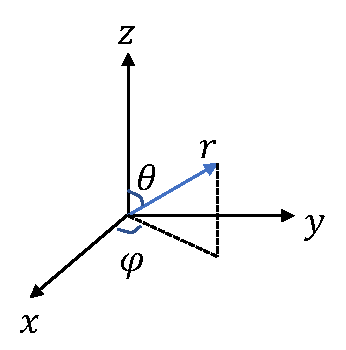
\includegraphics[width=4cm]{sph}
%\caption{}
%\label{}
\end{center}
\end{figure}

For a point in space, we use a ket $|\psi\rangle$ to represent it,
\begin{align*}
\begin{cases}x = r\sin\theta\cos\varphi \\ y = r\sin\theta\sin\varphi \\ z = r\cos\theta\end{cases} \Rightarrow r = \sqrt{x^{2} + y^{2} +z^{2}}
\end{align*}
now let's consider a rotation along $\hat{z}$ direction. Here $\varphi$ becomes $\varphi + d\varphi$, and $r,\theta$ remain the same. We have 
\begin{align}
|x,y,z\rangle \xrightarrow{\text{rotation}} |x', y', z'\rangle
\end{align}
and the corresponding
\begin{align}
(r,\theta,\varphi) \xrightarrow{\text{rotation}} (r, \theta, \varphi + d\varphi)
\end{align}
then we try to find out the expression of $x',y',z'$ in terms of $r,\theta,\varphi, d\varphi$
\begin{align}
\begin{cases}
x' = r\sin\theta\cos(\varphi+d\varphi) \simeq r\sin\theta\cos\varphi - r\sin\theta\sin\varphi d\varphi \\
y' = r\sin\theta\sin(\varphi+d\varphi) \simeq  r\sin\theta\sin\varphi + r\sin\theta\cos\varphi d\varphi \\
z' = r\cos\theta = z
\end{cases}
\Rightarrow \begin{cases}
x' = x - yd\varphi\\
y' = y + xd\varphi\\
z' = z
\end{cases}
\end{align}

On a spin-$\frac{1}{2}$ system, we have Pauli operators $\sigma_{x}, \sigma_{y}, \sigma_{z}$. In the $\sigma_{z}$ basis, we have
\begin{align}
\sigma_{x} = \begin{pmatrix}0&1\\1&0\end{pmatrix}, \sigma_{y} = \begin{pmatrix}0&-i\\i&0\end{pmatrix}, \sigma_{z} = \begin{pmatrix}1&0\\0&-1\end{pmatrix}
\end{align}
and
\begin{align}
[\sigma_{k}, \sigma_{l}] = 2i\varepsilon_{klm}\sigma_{m}, ~~\varepsilon_{klm} = \begin{cases}1 &\text{if } k,l,m \text{ in order}\\-1 &\text{if out of order}\end{cases}
\end{align}



\end{document}